\documentclass[10pt,twocolumn,letterpaper]{article}
%% Welcome to Overleaf!
%% If this is your first time using LaTeX, it might be worth going through this brief presentation:
%% https://www.overleaf.com/latex/learn/free-online-introduction-to-latex-part-1

%% Researchers have been using LaTeX for decades to typeset their papers, producing beautiful, crisp documents in the process. By learning LaTeX, you are effectively following in their footsteps, and learning a highly valuable skill!

%% The \usepackage commands below can be thought of as analogous to importing libraries into Python, for instance. We've pre-formatted this for you, so you can skip right ahead to the title below.

%% Language and font encodings
\usepackage[spanish,english]{babel}
\usepackage[utf8]{inputenc}
\usepackage[T1]{fontenc}
\usepackage{changepage}
%% Sets page size and margins
\usepackage[a4paper,top=3cm,bottom=2cm,left=3cm,right=3cm,marginparwidth=1.75cm]{geometry}
\usepackage{float}
%% Useful packages
\usepackage{amsmath}
\usepackage{graphicx}
\usepackage[colorinlistoftodos]{todonotes}
\usepackage[colorlinks=true, allcolors=blue]{hyperref}

%% Title
\title{
		%\vspace{-1in} 	
		\usefont{OT1}{bch}{b}{n}\\ 
		\huge Experimenting Q-Learning with Function Approximation \\
}

\usepackage{authblk}

\author{Syed Mohammed Umar Farooq}


	\affil{\small{Department of Electrical Engineering, IIT Madras}}


\begin{document}
\date{} 
\maketitle

\selectlanguage{english}
\begin{abstract}
This report explores the application of Q-learning on a specific state and reward model using both tabular and function approximation approaches. We begin by implementing vanilla Q-learning using a constant learning rate and the Robbins-Monro algorithm. We then extend the approach to function approximation, using polynomial functions to represent the Q-values, and apply both constant and Robbins-Monro learning strategies to study their impact on learning performance.

\end{abstract} 
\vspace{-5pt}
%{\textbf{Keywords} \\
%pick, 3-5, good, keywords}

\section{Introduction}
Q-learning is a widely used reinforcement learning algorithm that aims to learn the optimal action-value function, $Q(s, a)$, through interactions with an environment. In this project, we consider a specific reward model and state-transition setup and investigate the effect of different learning configurations on performance.
\vspace{2mm}

We begin with a baseline implementation of vanilla Q-learning, first using a constant learning rate, and then employing a Robbins-Monro learning rate schedule to allow for convergence over time. After establishing baseline behaviors, we explore Q-learning with function approximation. Specifically, we approximate the Q-function using polynomial features, allowing generalization across states. Both constant and Robbins-Monro learning rates are again tested in this setting.
\vspace{2mm}

Our goal is to understand the convergence behavior and learning efficiency of these methods under a controlled environment.


\section{Markov Decision Process (MDP)}

A Markov Decision Process (MDP) is a formal framework for modeling decision-making in situations where outcomes are partly random and partly under the control of an agent. It provides the foundation for most reinforcement learning (RL) problems.

MDPs are widely used in areas such as robotics, game theory, and economics—any domain involving sequential decisions under uncertainty. They enable agents to interact with an environment, learn from experience, and make decisions that maximize cumulative rewards.

\subsection*{Core Components of an MDP}

An MDP consists of the following components:

\begin{itemize}
    \item \textbf{Environment:} The external system with which the agent interacts. It defines the dynamics of the state transitions and rewards.
    
    \item \textbf{States ($\mathcal{S}$):} A set of all possible configurations in which the environment can exist.

    \item \textbf{Actions ($\mathcal{A}$):} The set of all possible actions the agent can take while in a given state.

    \item \textbf{Transition Model ($P$):} A probability distribution $P(s' \mid s, a)$ that describes the likelihood of reaching state $s'$ from state $s$ after taking action $a$.

    \item \textbf{Reward Function ($R$):} A mapping $R(s, a)$ that provides immediate feedback (positive or negative) to the agent for performing action $a$ in state $s$.

    \item \textbf{Policy ($\pi$):} A strategy or mapping from states to actions, $\pi: \mathcal{S} \rightarrow \mathcal{A}$. It defines the agent's behavior.

    \item \textbf{Discount Factor ($\gamma$):} A scalar $\gamma \in [0, 1)$ that determines the importance of future rewards relative to immediate ones.
\end{itemize}

\begin{figure}[h]
    \centering
    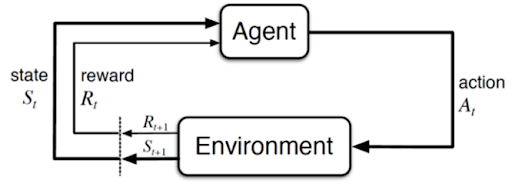
\includegraphics[width=0.45\textwidth]{MDP-model.png}
    \caption{A typical interaction in a Markov Decision Process (MDP).}
    \label{fig:mdp}
\end{figure}

At each time step, the agent observes the current state, selects an action based on its policy, receives a reward, and transitions to a new state as defined by the environment. The aim is to learn a policy that maximizes the expected cumulative reward over time.

This formulation lays the groundwork for learning algorithms like Q-learning, which estimates the optimal action-value function for guiding decisions.


\section{Value Functions and Bellman Equations}

In reinforcement learning, value functions estimate the expected return when following a policy. These functions help an agent evaluate the goodness of states and actions in a Markov Decision Process (MDP).

\subsection*{State-Value Function (\texorpdfstring{$V^\pi(s)$}{Vpi(s)})}

The state-value function under a policy $\pi$ is defined as the expected return starting from state $s$:
\[
V^\pi(s) = \mathbb{E}_\pi \left[ \sum_{t=0}^{\infty} \gamma^t R_{t+1} \mid S_0 = s \right]
\]

\subsection*{Action-Value Function (\texorpdfstring{$Q^\pi(s, a)$}{Qpi(s,a)})}

The action-value function represents the expected return starting from state $s$, taking action $a$, and thereafter following policy $\pi$:
\[
Q^\pi(s, a) = \mathbb{E}_\pi \left[ \sum_{t=0}^{\infty} \gamma^t R_{t+1} \mid S_0 = s, A_0 = a \right]
\]

\subsection*{Bellman Expectation Equations}

The Bellman expectation equations express value functions recursively in terms of immediate reward and the value of successor states:

For the state-value function:
\[
V^\pi(s) = \mathbb{E}_\pi \left[ R_{t+1} + \gamma V^\pi(S_{t+1}) \mid S_t = s \right]
\]

For the action-value function:
\begin{adjustwidth}{-1cm}{0cm}
$$
Q^*(s, a) = \mathbb{E} \big[ R_{t+1} + \gamma \max_{a'} Q^*(S_{t+1}, a') \,\big|\, S_t = s,\ A_t = a \big]
$$
\end{adjustwidth}

\subsection*{Bellman Optimality Equations}

The optimal value functions are defined in terms of the maximum expected return obtainable from each state or state-action pair:

For the optimal state-value function:
\[
V^*(s) = \max_a \mathbb{E} \left[ R_{t+1} + \gamma V^*(S_{t+1}) \mid S_t = s, A_t = a \right]
\]

For the optimal action-value function:
\[
Q^*(s, a) = \mathbb{E} \left[ R_{t+1} + \gamma \max_{a'} Q^*(S_{t+1}, a') 
\\
\mid S_t = s, A_t = a \right]
\]

The optimal policy $\pi^*$ can then be derived as:
\[
\pi^*(s) = \arg\max_a Q^*(s, a)
\]

\section{Dynamic Programming}

Dynamic Programming (DP) refers to a class of algorithms that solve complex problems by breaking them down into simpler subproblems and solving them recursively. In the context of Markov Decision Processes (MDPs), DP is used to compute the optimal value functions and policies when a complete model of the environment (i.e., transition probabilities and reward function) is known.

\subsection*{Policy Evaluation}
The goal of policy evaluation is to compute the value function $V^\pi(s)$ for a given policy $\pi$. This is done iteratively using the Bellman expectation equation:

\[
V_{k+1}(s) = \sum_{a} \pi(a|s) \sum_{s', r} p(s', r | s, a) \left[ r + \gamma V_k(s') \right]
\]

\subsection*{Policy Improvement}
Once the value function for a policy is known, we can improve the policy by acting greedily with respect to the current value function:

\[
\pi'(s) = \arg\max_a \sum_{s', r} p(s', r | s, a) \left[ r + \gamma V^\pi(s') \right]
\]

\subsection*{Policy Iteration}
Policy Iteration is an algorithm that alternates between policy evaluation and policy improvement until convergence to the optimal policy $\pi^*$.

\subsection*{Value Iteration}
Value Iteration combines policy evaluation and improvement into a single update:

\[
V_{k+1}(s) = \max_a \sum_{s', r} p(s', r | s, a) \left[ r + \gamma V_k(s') \right]
\]

This process is repeated until the value function converges to the optimal value function $V^*(s)$, from which the optimal policy can be derived.

\section{Q-Learning}

Q-Learning is a model-free, off-policy reinforcement learning algorithm that learns the optimal action-value function \( Q^*(s, a) \) through interaction with the environment.

\subsection*{Objective}

The Bellman optimality equation for \( Q^*(s, a) \) is:

\begin{adjustwidth}{-0.5cm}{0cm}
$$
Q^*(s, a) = \mathbb{E} \big[ R_{t+1} + \gamma \max_{a'} Q^*(S_{t+1}, a') \,\big|\, S_t = s,\ A_t = a \big]
$$
\end{adjustwidth}


Since the model is unknown, Q-learning approximates this using the update rule \cite{lecture10}:

\begin{adjustwidth}{-0.5cm}{0cm}
    $$
    Q(s, a) \leftarrow Q(s, a) + \alpha \big[ R + \gamma \max_{a'} Q(s', a') - Q(s, a) \big]
    $$
\end{adjustwidth}


\noindent where:
\begin{itemize}
    \item \( \alpha \) is the learning rate,
    \item \( \gamma \) is the discount factor,
    \item \( R \) is the received reward,
    \item \( s' \) is the next state.
\end{itemize}

\subsection*{Exploration vs. Exploitation: \(\varepsilon\)-Greedy Policy}

At each step, the agent:
\begin{itemize}
    \item Chooses a random action with probability \( \varepsilon \) (exploration),
    \item Chooses \( a = \arg\max_{a'} Q(s, a') \) with probability \( 1 - \varepsilon \) (exploitation).
\end{itemize}

\subsection*{Q-Learning Algorithm}

\begin{enumerate}
    \item Initialize \( Q(s, a) \) arbitrarily.
    \item For each episode:
    \begin{itemize}
        \item Start in initial state \( s \).
        \item Repeat:
        \begin{enumerate}
            \item Choose action \( a \) using \(\varepsilon\)-greedy policy.
            \item Observe reward \( R \) and next state \( s' \).
            \item Update:
            \[
            Q(s, a) \leftarrow Q(s, a) + \alpha \big[ R + \gamma \max_{a'} Q(s', a') - Q(s, a) \big]
            \]
            \item Set \( s \leftarrow s' \).
        \end{enumerate}
        until convergence.
    \end{itemize}
\end{enumerate}



\section{Function Approximation}

\begin{itemize}
    \item In tabular Q-learning, we maintain a separate value for every state-action pair. This becomes infeasible when the state or action space is large or continuous.
    
    \item \textbf{Function approximation} helps in generalizing across similar states or actions by learning a parameterized function to estimate the value function or Q-function.
    
    \item Instead of a table, we use a function $\hat{Q}(s, a; \boldsymbol{w})$ where $\boldsymbol{w}$ is a vector of parameters (e.g., weights in a neural network).
    
    \item According to \cite{lecture10} and \cite{ieee_qlearning}, the update rule of $\boldsymbol{w}$  :
    \[
    \boldsymbol{w} \leftarrow \boldsymbol{w} + \alpha \big( R + \gamma \max_{a'} \hat{Q}(s', a'; \boldsymbol{w}) - \hat{Q}(s, a; \boldsymbol{w}) \big) \nabla_{\boldsymbol{w}} \hat{Q}(s, a; \boldsymbol{w})
    \]
    
    \item This approach allows learning in problems with huge or continuous state-action spaces using methods like:
    \begin{itemize}
        \item Linear function approximation
        \item Non-linear approximators (e.g., neural networks)
        \item Tile coding, radial basis functions (RBF), etc.
    \end{itemize}
\end{itemize}

\subsection*{Linear Function Approximation}

In linear function approximation, the Q-value is represented as a linear combination of features:

\[
\hat{Q}(s, a; \boldsymbol{w}) = \boldsymbol{w}^\top \boldsymbol{\phi}(s, a)
\]

where \(\boldsymbol{\phi}(s, a)\) is the feature vector representing the state-action pair and \(\boldsymbol{w}\) is the weight vector.

The update rule for \(\boldsymbol{w}\) is:

\[
\boldsymbol{w} \leftarrow \boldsymbol{w} + \alpha \delta \nabla_{\boldsymbol{w}} \hat{Q}(s, a; \boldsymbol{w}) = \boldsymbol{w} + \alpha \delta \boldsymbol{\phi}(s, a)
\]

where the temporal-difference error \(\delta\) is

\[
\delta = R + \gamma \max_{a'} \hat{Q}(s', a'; \boldsymbol{w}) - \hat{Q}(s, a; \boldsymbol{w})
\]

This allows the algorithm to generalize Q-values across similar states and actions, facilitating learning in larger or continuous spaces.


\section{Experiments}

In this section, we detail the empirical experiments conducted to evaluate the performance of Q-learning under stochastic transitions. All experiments were implemented in \texttt{MATLAB}.

\subsection*{Environment Setup}

The environment is modeled with:

    
\textbf{State Space:} $\mathcal{S} = \{0, 1, \dots, p-1\}$, where $p$ is a natural number.
    
\textbf{Action Space:} $\mathcal{A} = \{0, 1, \dots, p-1\}$.
    
\textbf{Noise Space:} A uniformly distributed space $\mathcal{N} = \{0, 1, \dots, p-1\}$ with $\mathbb{P}(n = i) = \frac{1}{p}$ for all $i$.(We can use any probability distribution)


The transition dynamics are governed by:
\[
s_{t+1} = (s_t + a_t + n_t) \bmod p
\]
where $n_t$ is sampled from the noise space. This introduces stochasticity into an otherwise deterministic system.

All experiments were conducted using $\gamma = 0.9$ \& $p = 100$, meaning that each of the state, action, and noise spaces contained 100 elements.

\subsection*{Reward Model}

We define the reward function as:
\[
R(s_t, a_t) = s_t \cdot a_t
\]
This encourages the agent to select higher-value actions in higher-value states, enabling exploration of the full state-action landscape.

\subsection*{Vanilla Q-Learning}

The standard Q-learning algorithm updates the Q-values using the rule:
\begin{adjustwidth}{-0.75cm}{0cm}
    $$
    Q(s, a) \leftarrow Q(s, a) + \alpha \left[ R + \gamma \max_{a'} Q(s', a') - Q(s, a) \right]
    $$
\end{adjustwidth}
\paragraph{Case 1: Constant Learning Rate ($\alpha = 0.001$)}
\begin{figure}
    \centering
    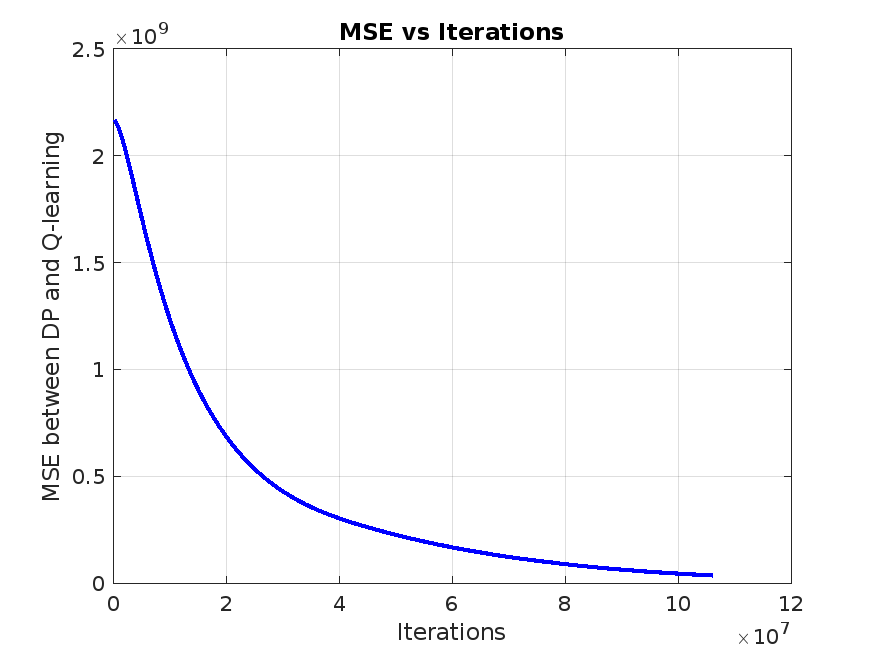
\includegraphics[width=1\linewidth]{MSE.png}
    \caption{MSE vs Iterations graph for Q-learning with constant learning rate}
    \label{fig:enter-label}
\end{figure}
In our setup:
\begin{itemize}
    \item $\alpha = 0.001$ was used as a constant learning rate.
    \item $\epsilon$-greedy exploration was applied with $\epsilon = 0.5$.
    \item \textbf{Convergence:} Achieved after $10^8$ iterations.
    \item \textbf{Time Taken:} 2137 seconds.
    \item \textbf{Accuracy:} Many Q-values were significantly different from the true values obtained via Dynamic Programming (DP).
    \item MSE between optimal values(calculated from DP) and Q-learning values at convergence is around $3.6 \times 10^7$. So the RMS error is around $6000$.
    \item From Figure 2, we can infer that convergence is very slow, even after $10^8$ iterations, the MSE is very high.
\end{itemize}

\subsection*{Q-Learning with Robbins-Monro Algorithm}

Conditions for the Robbins-Monro algorithm \cite{neuralq}:
\[
\sum_{t=1}^{\infty} \alpha_t = \infty, \quad \sum_{t=1}^{\infty} \alpha_t^2 < \infty,
\]

We also evaluated a variant using a diminishing learning rate schedule inspired by the Robbins-Monro conditions. For each state-action pair $(s,a)$, the learning rate was updated as:
\[
\alpha(s,a) = \frac{\alpha_0}{1 + N(s,a)}
\]
where $N(s,a)$ counts how often a state-action pair has been visited.

This choice is motivated by the need to balance initial exploration with eventual convergence \cite{lecture10}. At the beginning of learning, higher learning rates help the agent adjust quickly to new information. As more samples are collected for a given $(s,a)$ pair, the learning rate decreases, reducing the effect of noise and stabilizing the Q-value updates.

This learning rate satisfies the Robbins-Monro conditions.

The update rule becomes:
\begin{adjustwidth}{-2cm}{0cm}
    $$
    Q(s, a) \leftarrow Q(s, a) + \frac{\alpha_0}{1 + N(s,a)} \left[ R + \gamma \max_{a'} Q(s', a') - Q(s, a) \right]
    $$
\end{adjustwidth}


This method stabilizes convergence by reducing the step size as more data is gathered, especially beneficial in noisy environments.

\begin{figure}
    \centering
    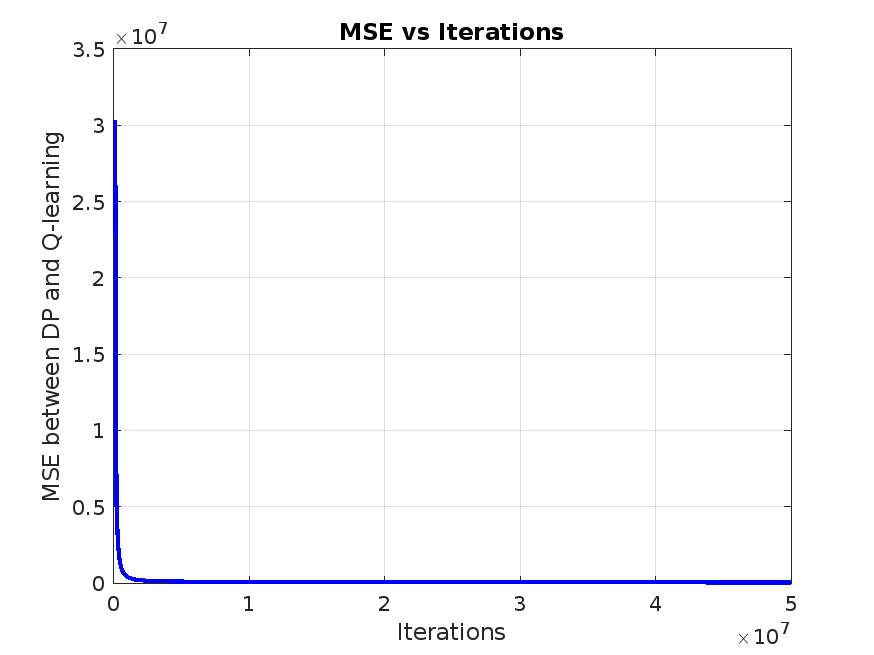
\includegraphics[width=1\linewidth]{MSE_vs_Iterations.png}
    \caption{MSE vs Iterations graph for Q-learning with Robbins-Monro learning rate}
    \label{fig:enter-label}
\end{figure}
In our setup:
\begin{itemize}
    \item $\alpha_0$ = 1.
    \item \textbf{Convergence:} Achieved after $5 \times 10^7$ iterations.
    \item \textbf{Time Taken:} 996 seconds.
    \item \textbf{Accuracy:} Most Q-values are near to those computed by DP.
    \item MSE between optimal values(calculated from DP) and Q-learning values at convergence is around 39611. So the RMS error is around 199.
    \item From Figure 3, we can infer that convergence is very fast.
\end{itemize}

\subsection*{Implementation Notes}

The agent starts from a random initial state and explores the environment using $\epsilon$-greedy policy. Transitions are sampled according to the uniform noise distribution. The algorithm halts when the maximum change in Q-values falls below a threshold ($10^{-6}$).

\subsection*{Results}

From our experiments, the Q-learning variant using the Robbins-Monro learning rate schedule demonstrated faster convergence and required less computation time compared to the standard Q-learning algorithm with a constant learning rate. Additionally, the diminishing step size led to more stable updates in the presence of noise, resulting in Q-values that were closer to those obtained via Dynamic Programming. With increasing number of iterations the MSE can be reduced.

\begin{table*}[t]
\noindent
\begin{minipage}{\linewidth}
\raggedright
\caption{Runtime, Convergence and RMS error Comparison}
\label{tab:runtime}
\begin{tabular}{|l|c|c|c|}
\hline
\textbf{Algorithm} & \textbf{Runtime (s)} & \textbf{Convergence at} & \textbf{RMS Error} \\
\hline
Vanilla Q-Learning & 2137 & $1 \times 10^{8}$  & 6000\\
Q-Learning + Robbins-Monro & 996 & Not Converged & 199\\
Function Approximation (Constant Learning rate) & 1115 & $5 \times 10^{7}$  & 6000\\
Function Approximation (Robbins-Monro) & 570 & $3 \times 10^{7}$  & 1673\\
\hline
\end{tabular}
\end{minipage}
\end{table*}


\subsection*{Q-Learning with Linear Function Approximation}

To scale Q-learning to large MDPs efficiently, we implemented a linear function approximation approach:
$$
\hat{Q}(s, a; w) = \phi(s, a)^T w
$$
where:
\\
 $\phi(s, a)$ is the feature vector representing $(s,a)$,
 $w$ is the weight vector of learnable parameters.

\subsubsection*{Feature Vector Construction}

Before computing features, both the state and action values were normalized to lie in the interval $[0,1]$:
\[
\tilde{s} = \frac{s}{p - 1}, \quad \tilde{a} = \frac{a}{p - 1}
\]

We then constructed a feature vector using a 10th-degree polynomial(we can use polynomial of any degree except 1) basis over the normalized state-action pair $(\tilde{s}, \tilde{a})$:
\begin{adjustwidth}{0cm}{0cm}
    $$
    \phi(s, a) = [1,\ \tilde{s},\ \tilde{a},\ \tilde{s}^2,\ \tilde{s}\tilde{a},\ \tilde{a}^2,\ \ldots,\ \tilde{s}^{10},\ \tilde{s}^9\tilde{a},\ \ldots,\ \tilde{a}^{10}]^T
    $$
\end{adjustwidth}

This resulted in a total of 66 features, covering all monomials of total degree up to 10 in two variables.

For polynomial of degree $k$, the number of features are $(k+1)(k+2)/2$.

The reason for not using a polynomial of degree 1 as the feature representation stems from the structure of the action-value function as defined by the Bellman Expectation Equation:

\begin{adjustwidth}{0cm}{0cm}
$$
Q^*(s, a) = \mathbb{E} \big[ R_{t+1} + \gamma \max_{a'} Q^*(S_{t+1}, a') \,\big|\, S_t = s,\ A_t = a \big]
$$
\end{adjustwidth}

In our setting, the reward is defined as $R_{t+1} = s_t.a_t$, which is deterministic and depends directly on the current state and action. Substituting this into the equation yields:
\begin{adjustwidth}{-1cm}{0cm}
$$
Q^*(s, a) = s_t.a_t + \mathbb{E} [\gamma \max_{a'} Q^*(S_{t+1}, a') \,\big|\, S_t = s,\ A_t = a \big]
$$
\end{adjustwidth}

A degree-1 polynomial feature vector, \( \phi(s, a) = [1,\ \tilde{s},\ \tilde{a}] \), includes only linear terms and omits the crucial interaction term \( s \cdot a \). Since \( Q^*(s, a) \) depends explicitly on this term, degree-1 features are insufficient to capture its structure. This motivates the use of higher-order or custom features that include \( s \cdot a \).

\subsubsection*{Learning Algorithm and Update Rule}

The Q-learning update was performed using stochastic gradient descent on the Bellman residual:
$$
\boldsymbol{w}_{t+1} = \boldsymbol{w}_t + \alpha_t \cdot \delta_t \cdot \phi(s_t, a_t)
$$
where:
\\
$\delta_t = r_t + \gamma \max_{a'} \hat{Q}(s_{t+1}, a'; \theta_t) - \hat{Q}(s_t, a_t; \boldsymbol{w}_t)$ is the TD error,
\\
$\alpha_t$ is the learning rate at time $t$.
\\
We tested two learning rate schedules:

    
- \textbf{Constant Learning Rate:} $\alpha_t = 0.001$
    
- \textbf{Robbins-Monro Schedule:} $\alpha_t = \frac{1}{N(s_t, a_t)}$


The Robbins-Monro condition requires:
$$
\sum_{t=1}^\infty \alpha_t = \infty, \quad \sum_{t=1}^\infty \alpha_t^2 < \infty
$$

\subsubsection*{Initialization and Exploration Strategy}

- Weight vector $\theta$ was initialized randomly with small values: $\theta \sim \mathcal{N}(0, 0.1^2)$
- We used $\epsilon$-greedy exploration with $\epsilon = 0.6$.
- Discount factor was set to $\gamma = 0.90$

\subsection*{Implementation Notes}
The agent starts from a random initial state and explores the environment using $\epsilon$-greedy policy. Transitions are sampled according to the uniform noise distribution. The algorithm halts when the maximum change in weight vector $w$ falls below a threshold ($10^{-6}$).

\subsubsection*{Results with Function Approximation}

We evaluated the performance of Q-learning using 10-degree polynomial function approximation (66 features per $(s,a)$ pair).

\paragraph{Case 1: Constant Learning Rate ($\alpha = 0.001$)}
\begin{figure}
    \centering
    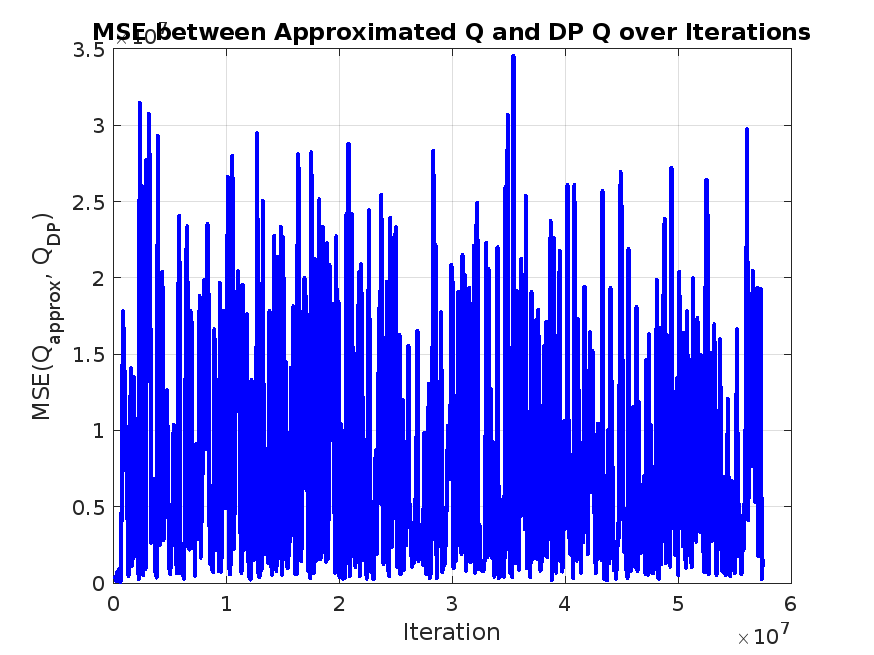
\includegraphics[width=1\linewidth]{Q_MSE_vs_Iteration.png}
    \caption{MSE($10^7$) vs Iterations graph for Function Approximation with constant learning rate}
    \label{fig:enter-label}
\end{figure}
\begin{itemize}
    \item \textbf{Convergence:} From thresold limit, it will run around upto $5\times10^7$ iterations, but observing figure 4, due to the spikes in the plot, it is not converged.
    \item \textbf{Time Taken:} 1115 seconds.
    \item \textbf{Accuracy:} Learned Q-values were not close to those from DP.
    \item MSE between optimal values(calculated from DP) and Q-function approximation values upto $5\times10^7$ iterations is around $3.5 \times 10^7$, the RMS error will be around 6000.
\end{itemize}

\paragraph{Case 2: Robbins-Monro Learning Rate}
\begin{figure}
    \centering
    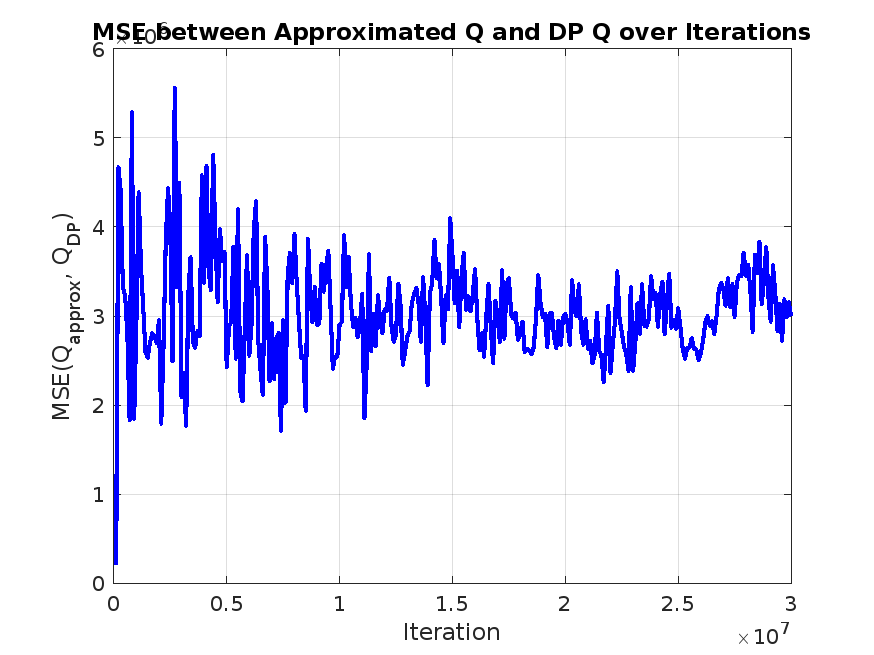
\includegraphics[width=1\linewidth]{MSE_rb_fa.png}
    \caption{MSE($10^6$) vs Iterations graph for Q-learning with Robbins-Monro learning rate}
    \label{fig:enter-label}
\end{figure}
According to \cite{ieee_qlearning}, a condition that implies the convergence of this approximation method with probability 1 is:
\[
\|\phi(s, a)\|_2 \leq 1 \quad \forall (s,a)
\]

Since our initial feature vector \(\phi(s,a)\) is a 10th-degree polynomial basis, we normalize it to satisfy this condition by defining:
\[
\phi(s, a) \leftarrow \frac{\phi(s, a)}{\|\phi(s, a)\|_2} \quad \forall (s,a)
\]

\begin{itemize}
    \item \textbf{Convergence:} Achieved after $3 \times 10^7$ iterations.
    \item \textbf{Time Taken:} 570 seconds.
    \item \textbf{Accuracy:} Many Q-values were closer to DP results than with constant learning rate.
    \item MSE between optimal values(calculated from DP) and Q-function approximation is around $2.8\times10^6$, the RMS error is around 1673.
    \item From Figure 5, we can infer that convergence is very fast.
\end{itemize}

\paragraph{Observation:}

The Robbins-Monro adaptive learning rate scheme not only improved convergence stability but also accelerated training overall. Initially, the higher step sizes enabled the algorithm to explore and update Q-values more aggressively. As the number of visits to each state-action pair increased, the step sizes naturally decreased, leading to more stable and smoother convergence by reducing the variance introduced by noise. In contrast, function approximation with a constant learning rate lacks such adaptivity, and convergence is not guaranteed.

\subsection*{With Learning Rate \(\alpha_t = \frac{1}{t}\)}

This learning rate satisfies the Robbins-Monro conditions:
\[
\sum_{t=1}^\infty \alpha_t = \infty, \quad \sum_{t=1}^\infty \alpha_t^2 < \infty.
\]

\begin{itemize}
    \item Experiments show that using \(\alpha_t = \frac{1}{t}\) leads to slow convergence and requires a large number of iterations for both Q-learning and function approximation.
    \item Since the learning rate decreases over time, state-action pairs \((s,a)\) that are visited infrequently may not receive sufficient updates, hindering proper value learning.
\end{itemize}


\subsubsection*{Discussion}

Function approximation significantly reduces memory usage by replacing the $100 \times 100$ Q-table with just 66 weights, enabling generalization across unseen state-action pairs and scaling to larger problems.

Key observations:
\begin{itemize}
    \item The 10\textsuperscript{th}-degree polynomial features effectively approximated the true Q-values.
    \item Robbins-Monro learning takes more time to converge on increasing $p$ or on increasing $k$, but it gives stable convergence than constant rates.
    \item Learning rates must be chosen carefully. For instance, while the Robbins-Monro condition (e.g., $\alpha_t = 1/t$) guarantees convergence, such learning rates can lead to slower convergence in practice.
    \item Q-leaning using Robbins-Monro algorithm can achieve faster convergence. 
    
\end{itemize}

\subsubsection*{Conclusion}

\begin{itemize}
    \item Linear function approximation using 10-degree polynomial features offers a compact and effective means to generalize across large state-action spaces.
    \item The Robbins-Monro algorithm demonstrated significantly faster and more accurate convergence than the fixed learning rate method, highlighting the benefits of adaptive learning rates in stochastic environments and large-scale Markov Decision Processes.
    \item Function approximation remains a powerful approach for scaling reinforcement learning to large domains and is even faster than vanilla Q-learning.
\end{itemize}

\begin{thebibliography}{9}

\bibitem{lecture10}
D. Katselis, “Stochastic Approximation and Robbins-Monro Algorithm,” \textit{ECE 586: Vector Space Methods}, University of Illinois at Urbana-Champaign. [Online]. Available: \url{https://katselis.web.engr.illinois.edu/ECE586/Lecture10.pdf}

\bibitem{ieee_qlearning}
A. Rajeswaran, S. Ghotra, B. Ravindran, and S. Bhatnagar, “Finite-time analysis of the stochastic approximation variant of TD learning,” \textit{IEEE Transactions on Automatic Control}, vol. 60, no. 4, pp. 1010–1015, 2015. [Online]. Available: \url{https://ieeexplore.ieee.org/stamp/stamp.jsp?tp=&arnumber=7068926}

\bibitem{neuralq}
C. J. C. H. Watkins and P. Dayan, “Q-learning,” in \textit{Advances in Neural Information Processing Systems (NeurIPS)}, vol. 3, 1992. [Online]. Available: \url{https://proceedings.neurips.cc/paper_files/paper/2001/file/6f2688a5fce7d48c8d19762b88c32c3b-Paper.pdf}

\end{thebibliography}


\end{document}